\chapter[State of the Art]{State of the Art of the Technology Used or Applied in this Thesis}

In recent years, computing has undergone significant evolution, reaching a point where improving the hardware of traditional devices presents considerable challenges. This has driven research in quantum computing, a technology that promises to revolutionize the field by enabling much more efficient calculations and superior processing capabilities. In applications such as molecular simulation, quantum computing has proven to be remarkably more efficient than classical computing, justifying investment in its development.

However, one of the main obstacles of quantum computing is the high cost associated with its devices. To run programs on a quantum computer, it must operate at extremely low temperatures, close to 0.1 Kelvin, which significantly increases the cost and technical complexity. Therefore, methods are being investigated to improve and optimize these devices, making them more accessible and viable for broader use.

Currently, one of the most practical ways to harness quantum computing's potential is through \textbf{quantum simulation}. Quantum simulation allows us to study complex quantum systems using either quantum simulators or classical computers. By emulating the behavior of quantum systems, we can explore quantum algorithms and applications effectively without necessarily requiring a fully functional quantum computer.

In this project, we focus on the operation of quantum simulators applied to molecular simulation, an area where quantum computing offers significant advantages. The main objective is to develop a program capable of simulating different molecules in a simple and efficient manner.

To this end, we will review the basic concepts of quantum mechanics that are essential to understand the fundamentals and potential of quantum computing, and explore the techniques of quantum simulation that allow us to harness quantum computing capabilities even with current technological limitations.

\section{Quantum Simulation}

Quantum simulation has emerged as an advanced and essential technique for studying complex quantum systems, especially those that are inaccessible or present great challenges for direct analysis using classical methods. Based on the proposal of Richard Feynman, who postulated that a computer built from quantum elements could overcome the limitations of classical computers in simulating quantum phenomena, quantum simulation has progressed significantly. It encompasses both digital and analog simulations and has expanded its applicability in various scientific areas.

There are mainly two approaches in quantum simulation: \textbf{Digital Quantum Simulation (DQS)} and \textbf{Analog Quantum Simulation (AQS)}. DQS employs the quantum circuit model, where systems are represented by qubits that evolve through quantum gates to reproduce the dynamics of the target system. This approach is universal, as it can, in principle, simulate any quantum system, although not always efficiently. On the other hand, AQS involves creating a quantum system that directly emulates the Hamiltonian of the system under study, allowing certain properties of the simulated system, such as time evolution, to be reproduced approximately. This method is particularly useful when a qualitative representation is required rather than high precision.

In addition to these approaches, there are algorithms inspired by quantum information theory that facilitate the classical simulation of quantum systems. Techniques such as \textbf{Matrix Product States (MPS)} and \textbf{Projected Entangled Pair States (PEPS)} allow representing particle systems on classical computers more efficiently than standard classical methods, optimizing the calculation of properties of complex quantum systems.

The applications of quantum simulation are broad and encompass multiple scientific fields. In condensed matter physics, it allows the study of models such as the Hubbard model and quantum phase transitions, fundamental for understanding phenomena like superconductivity. In quantum chemistry, it facilitates the calculation of molecular energies and complex chemical reactions. In high-energy physics and cosmology, it emulates particles in high-energy fields and cosmological phenomena. Furthermore, quantum simulation is instrumental in the analysis of open quantum systems and in the investigation of quantum chaos, allowing exploration of interactions with the environment and chaotic dynamics in the quantum realm.

However, quantum simulation faces significant challenges related to the precise control of the quantum simulator systems and the management of decoherence and errors, which can affect the accuracy of the results. The amount of required resources, such as the number of qubits and quantum gates, also depends on the size and complexity of the system to be simulated. It is estimated that quantum simulators require between 40 and 100 qubits to surpass the computational power of classical computers in specific problems. Despite these challenges, technological advances continue to improve the viability and efficiency of quantum simulation, promising to transform research in natural sciences and expand our understanding of quantum phenomena.

\section{Key Concepts in Quantum Mechanics}

It is essential to understand the difference between bits in classical computing and qubits in quantum computing to delve into this new technological paradigm.

In classical computing, the basic unit of information is the \textbf{bit}, which can take the value of 0 or 1. These bits are the foundation upon which conventional computers operate, processing information through combinations of these binary states.

In contrast, quantum computing uses the \textbf{qubit} or quantum bit as its basic unit. Unlike the classical bit, a qubit can exist in a superposition of states, meaning it can simultaneously represent the values 0 and 1 thanks to the principle of superposition in quantum mechanics. This property, along with phenomena such as quantum entanglement and interference, allows quantum computers to process information exponentially more efficiently for certain problems.

\begin{figure}[H]
    \centering
    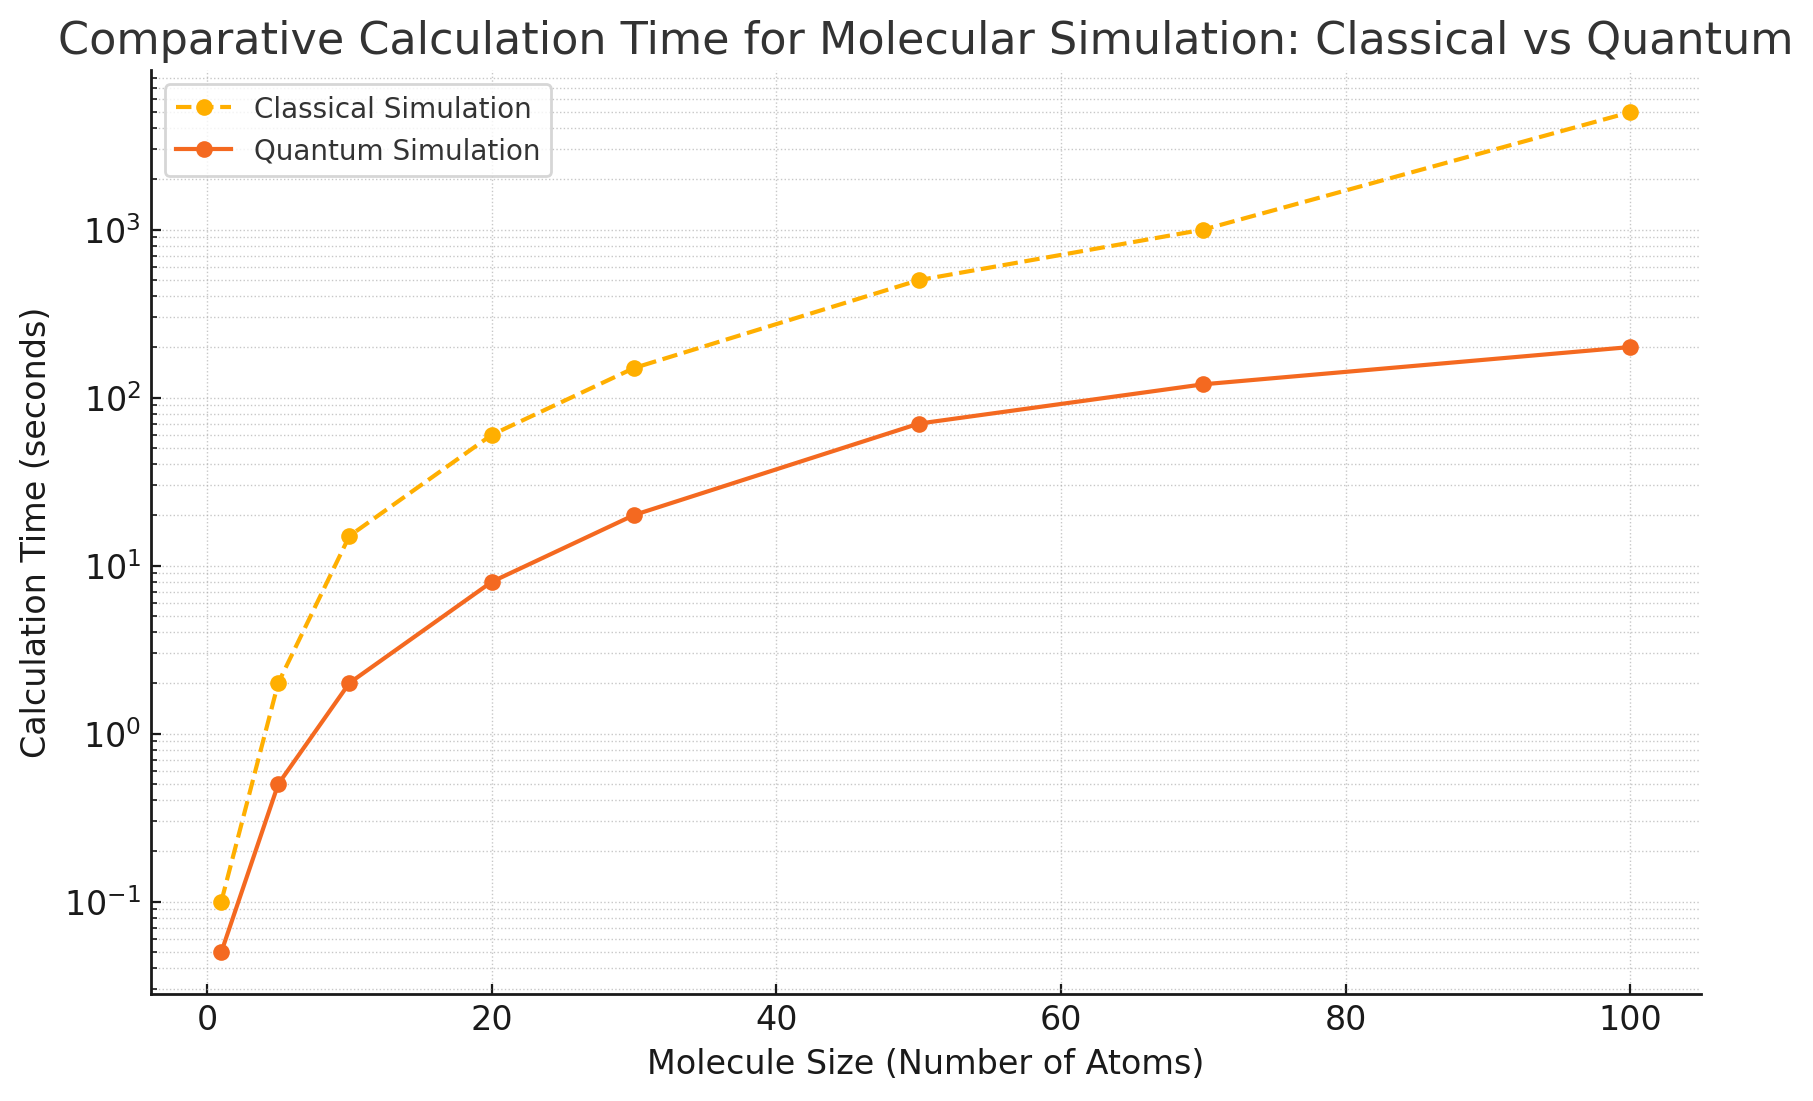
\includegraphics[width=0.8\textwidth]{img/bit_vs_qbit.png}
    \caption{Comparison of computation time for molecular simulations: classical vs quantum.}
    \label{fig:bit_vs_qubit}
\end{figure}

Understanding how qubits operate and their differences from classical bits is essential to appreciate the revolutionary potential of quantum computing.

\subsection{Qubit}

The \textbf{qubit} is the basic unit of information in quantum computing. While the classical bit can only be in one of two states (0 or 1), a qubit can be in a superposition of both states simultaneously. This is due to the principle of quantum superposition, one of the fundamental characteristics of quantum mechanics.

Mathematically, a qubit is represented as a linear combination of the basis states $\ket{0}$ and $\ket{1}$:

\[
\ket{\psi} = \alpha\ket{0} + \beta\ket{1}
\]

where $\alpha$ and $\beta$ are complex numbers that satisfy the normalization condition $|\alpha|^2 + |\beta|^2 = 1$. These coefficients indicate the probability amplitudes of finding the qubit in the states $\ket{0}$ or $\ket{1}$ upon measurement.

In addition to superposition, qubits can exhibit \textbf{quantum entanglement}, a property that allows creating strong correlations between qubits that cannot be explained by classical physics. Entanglement is essential for the computational power of quantum computers, as it enables processing and storing an exponentially larger amount of information than classical systems.

For example, while a classical system of $n$ bits can represent one of $2^n$ possible state combinations, a quantum system of $n$ qubits can represent a superposition of all those combinations simultaneously. This capability is what allows quantum computers to tackle complex problems more efficiently.

However, manipulating and maintaining qubits is a significant technical challenge. Qubits are extremely sensitive and can be affected by interactions with the environment, leading to \textbf{quantum decoherence}. To minimize this effect and preserve quantum properties, it is necessary to keep systems in controlled conditions, such as very low temperatures, close to absolute zero.

\subsection{Quantum Superposition}

\textbf{Quantum superposition} allows a quantum system to exist in multiple states simultaneously until a measurement is performed. This characteristic is key to the functioning of quantum computers, as it enables processing a large amount of information in parallel.

In quantum systems, superposition is combined with \textbf{quantum interference}, where the probability amplitudes of states can reinforce or cancel each other out. This phenomenon is exploited in quantum algorithms to increase the probability of obtaining the correct result. For example, in Grover's algorithm, constructive interference amplifies the probability of the desired state, significantly improving the efficiency of searching for elements in an unsorted database.

Superposition is especially useful in simulating complex molecular systems. Quantum computers can naturally model the superpositions of electronic states in molecules, which is crucial for studying chemical reactions and molecular properties that are difficult to address with classical methods due to the exponential growth of computational resources required.

\subsection{Quantum Decoherence}

\textbf{Quantum decoherence} is one of the main challenges in quantum computing. It refers to the loss of a system's quantum properties, such as superposition and entanglement, due to unwanted interactions with the environment. This loss causes the quantum system to transition toward classical behavior, affecting the accuracy and reliability of quantum calculations.

Qubits are extremely sensitive to external disturbances, such as electromagnetic fluctuations, vibrations, and temperature changes. These interactions can cause quantum states to mix with those of the environment, leading to a loss of coherence that is irreversible and degrades the stored quantum information.

To mitigate the effects of decoherence, various strategies are implemented:

\begin{itemize}
    \item \textbf{System Isolation}: Designing physical systems that minimize unwanted interactions with the environment, using materials and techniques that protect qubits from external disturbances.
    \item \textbf{Quantum Error Correction}: Implementing error correction codes that allow detecting and correcting errors without directly measuring the qubit's state, thereby preserving quantum information.
    \item \textbf{Dynamic Control}: Applying techniques such as pulse refocusing and dynamic pulse sequences that actively compensate for disturbances and extend the coherence time of qubits.
\end{itemize}

Controlling and mitigating decoherence are essential for the advancement of quantum computing and its application in areas like molecular simulation, where the precision of calculations is fundamental.

\section{The Hamiltonian in Quantum Mechanics}

The Hamiltonian is a fundamental concept originating from classical mechanics, introduced by William Rowan Hamilton in 1833. Hamiltonian mechanics is a reformulation of classical mechanics that provides powerful tools for studying the dynamics of systems. The Hamiltonian function represents the total energy of the system, expressed in terms of generalized coordinates and momenta, and is given by the sum of the kinetic and potential energies.

In quantum mechanics, the \textbf{Hamiltonian operator} plays a central role in describing the energy and time evolution of quantum systems. It represents the total energy of the system, including both kinetic and potential energies, and is essential for formulating the Schrödinger equation.

\subsection{Mathematical Definition}

The Hamiltonian operator, commonly denoted as \( \hat{H} \), is a self-adjoint operator acting on the Hilbert space associated with the quantum system. For a single particle in one dimension, the Hamiltonian is expressed as:

\[
\hat{H} = \hat{T} + \hat{V}
\]

where:

\begin{itemize}
    \item \( \hat{T} \) is the kinetic energy operator.
    \item \( \hat{V} \) is the potential energy operator.
\end{itemize}

In terms of the position \( \hat{x} \) and momentum \( \hat{p} \) operators, these are defined as:

\[
\hat{T} = \frac{\hat{p}^2}{2m} = -\frac{\hbar^2}{2m} \frac{d^2}{dx^2}
\]

\[
\hat{V} = V(\hat{x})
\]

Here, \( m \) is the mass of the particle, \( \hbar \) is the reduced Planck constant, and \( V(\hat{x}) \) is the potential energy function depending on position.

\subsection{Role in the Schrödinger Equation}

The Hamiltonian is central to the Schrödinger equation, which describes how the quantum state of a system evolves over time. The time-dependent Schrödinger equation is expressed as:

\[
i\hbar \frac{\partial}{\partial t} |\psi(t)\rangle = \hat{H} |\psi(t)\rangle
\]

where \( |\psi(t)\rangle \) is the state vector of the system at time \( t \). For time-independent systems, the Schrödinger equation reduces to the eigenvalue equation:

\[
\hat{H} |\psi\rangle = E |\psi\rangle
\]

Here, \( E \) represents the eigenvalues of the Hamiltonian, corresponding to the allowed energy levels of the system, and \( |\psi\rangle \) are the associated eigenstates.

\subsection{Hamiltonian in Multi-Particle Systems}

For systems with multiple particles, the Hamiltonian includes additional terms representing interactions between particles. For example, for a system of two particles, the Hamiltonian is expressed as:

\[
\hat{H} = \hat{T}_1 + \hat{T}_2 + \hat{V}_1 + \hat{V}_2 + \hat{V}_{12}
\]

where:

\begin{itemize}
    \item \( \hat{T}_1 \) and \( \hat{T}_2 \) are the kinetic energy operators of particles 1 and 2, respectively.
    \item \( \hat{V}_1 \) and \( \hat{V}_2 \) are the individual potential energy operators.
    \item \( \hat{V}_{12} \) represents the potential interaction between the two particles.
\end{itemize}

\subsection{Importance in Quantum Simulations}

In quantum simulations, especially in algorithms like the Variational Quantum Eigensolver (VQE), the Hamiltonian is decomposed into a sum of simpler terms, often expressed in terms of Pauli operators. This decomposition facilitates implementation on quantum circuits and allows estimating the system's energy through measurements on qubits.

Understanding the structure and properties of the Hamiltonian is essential for modeling and simulating quantum systems, as it determines the possible energies and dynamics of the system under study.

\section{Algorithms}

Once we have understood the basic concepts, we focus on the quantum algorithms used in particle simulation. These algorithms make use of quantum logic gates, which are detailed in Appendix~\ref{appendices:LogicGates}.

\subsection{VQE: Variational Quantum Eigensolver}

The VQE is a hybrid quantum-classical algorithm designed to find the minimum energy of a quantum system, such as a molecule. This algorithm combines quantum state preparation with classical optimization. It leverages the quantum properties of qubits to find the ground state of the molecule more rapidly, followed by classical optimization to refine the solution.

\subsubsection*{Stages of the Algorithm}
El VQE  is based on the variational principle, which states that the expected energy of any approximate state \( |\psi(\theta)\rangle \) is always greater than or equal to the energy of the true ground state \( E_0 \):

\[
E(\theta) = \langle \psi(\theta) | H | \psi(\theta) \rangle \geq E_0
\]

\paragraph{1. Quantum State Preparation}

A parameterized quantum circuit known as an \textit{ansatz} is used, defined by a set of adjustable parameters \(\vec{\theta}\). This circuit applies a sequence of quantum gates, such as rotations and entangling gates, to generate a quantum state:

\[
|\psi(\vec{\theta})\rangle
\]

\paragraph{2. Measurement of the Expected Energy}

For a given quantum state \(|\psi(\vec{\theta})\rangle\), the expected energy of the system under a Hamiltonian \(H\) is measured:

\[
E(\vec{\theta}) = \langle \psi(\vec{\theta}) | H | \psi(\vec{\theta}) \rangle
\]

The Hamiltonian \(H\) is decomposed into terms of Pauli operators representing the electronic and nuclear interactions in the system.

\paragraph{3. Classical Optimization}

The parameters \(\vec{\theta}\) are iteratively adjusted using a classical optimizer to minimize \(E(\vec{\theta})\).

\paragraph{4. Iteration of the Process}

The steps of state preparation, measurement, and optimization are repeated until \(E(\vec{\theta})\) converges to a minimum value. This value corresponds to the ground state energy of the system.

\subsection{Adaptive Circuits}

\textbf{Adaptive circuits} allow optimizing the design of quantum circuits for specific problems. They dynamically adjust their structure based on feedback and optimization criteria during the execution process.

An example is found in \textit{Variational Quantum Algorithms} (VQA), which use classical optimization techniques to adjust the parameters of a quantum circuit and minimize a cost function. These algorithms are especially useful in current quantum devices, which are noisy and of limited size (NISQ).

For more information and practical examples on adaptive circuits:

\url{https://pennylane.ai/qml/demos/tutorial_adaptive_circuits/}

\section{Optimizers}

In the realm of quantum simulation algorithms like the \textbf{Variational Quantum Eigensolver} (VQE), optimizers are essential components that facilitate the minimization of the expected energy of a quantum system. Following the preparation of quantum states and the measurement processes described earlier, optimizers are employed in the classical computation stage to adjust the parameters of the quantum circuit, known as the \textit{ansatz}.

The theoretical purpose of optimizers in this project is to solve a continuous optimization problem. They aim to find the optimal set of parameters \(\vec{\theta}\) that minimize the cost function \(E(\vec{\theta})\), which represents the expectation value of the Hamiltonian \(H\) with respect to the quantum state \(| \psi(\vec{\theta}) \rangle\):

\[
E(\vec{\theta}) = \langle \psi(\vec{\theta}) | H | \psi(\vec{\theta}) \rangle
\]

Optimizers utilize mathematical techniques to navigate the high-dimensional parameter space effectively. Depending on the specific characteristics of the problem, different optimization methods can be employed:

\begin{itemize}
    \item \textbf{Gradient-based methods}: These methods compute the gradient of the cost function with respect to the parameters and use this information to guide the search towards the minimum energy. Examples include gradient descent and its variants.
    \item \textbf{Gradient-free methods}: In cases where calculating the gradient is impractical or the cost function is noisy, gradient-free methods like Nelder-Mead or COBYLA can be used.
    \item \textbf{Second-order methods}: These methods, such as the BFGS algorithm, approximate the second derivatives (Hessian) of the cost function to achieve faster convergence.
\end{itemize}

Within the iterative loop of the VQE algorithm, the optimizer updates the parameters \(\vec{\theta}\) after each quantum measurement based on the chosen optimization strategy. This process continues until convergence is achieved, meaning the expected energy \(E(\vec{\theta})\) reaches a minimum value that approximates the ground state energy of the system.

Integrating optimizers into the quantum-classical workflow is crucial because they connect quantum computations with classical numerical methods. They enable effective exploration of the parameter space, addressing challenges such as multiple local minima and flat regions in the energy landscape that are inherent in quantum systems.

By employing appropriate optimization techniques, this project aims to enhance the efficiency and accuracy of molecular simulations. Optimizers play a pivotal role in leveraging the capabilities of quantum computing to achieve results that are difficult to obtain with classical computational methods alone, thus contributing to the advancement of quantum simulation despite current technological limitations.





